\titleframe

%%%%%%%%%%%%%%%%%%%%%%%%%%%%%%%%%%%%%%%%%%%%%%%%%%%%%
%%%%%%%%%%%%%%%%%%%%%%%%%%%%%%%%%%%%%%%%%%%%%%%%%%%%%

\section{Sobre la materia - Datos útiles}

%%%%%%%%%%%%%%%%%%%%%%%%%%%%%%%%%%%%%%%%%%%%%%%%%%%%%

\begin{frame}{Sobre la materia}
  Como primer materia de la carrera enfocada al área de programación 
  informática, la presente tiene por objetivo introducir a los/las estudiantes
  a los conceptos básicos de informática y lógica requeridos para las
  subsiguientes materias de la carrera.
  \jump
  También tiene por objetivo introducirlos a prácticas que le serán útiles
  tanto en la carrera como en la vida universitaria en general.
  \jump
  Para muchos, algunos conceptos pueden parecer muy sencillos y hasta ya
  conocidos, otros pueden ser nuevos. Recomendamos no confiarse y seguir
  con atención todas las clases.
\end{frame}

%%%%%%%%%%%%%%%%%%%%%%%%%%%%%%%%%%%%%%%%%%%%%%%%%%%%%

\begin{frame}{Sitio web}
  La materia cuenta con una página web
  \jump
  \colored{\href{http://elementosdeprogramacionylogica.web.unq.edu.ar}{http://elementosdeprogramacionylogica.web.unq.edu.ar}}
  \jump
  En este sitio pueden encontrar:
  \begin{itemize}
    \item Todas las diapositivas teóricas de la materia.
    \item Guías de ejercicios prácticos.
    \item Fechas de exámenes actualizadas.
    \item Recursos útiles para la materia.
    \item Otra información relevante.
  \end{itemize}
  \emptyline
  \bolder{¡¡¡Hay que visitarla periódicamente!!!}
\end{frame}

%%%%%%%%%%%%%%%%%%%%%%%%%%%%%%%%%%%%%%%%%%%%%%%%%%%%%

\begin{frame}{Lista de correo}
  Todos deben estar subscriptos a la lista de correos de la materia.
  La suscripción es obligatoria para poder rendir los exámenes.
  \jump
  En la lista de correo van a aparecer cosas como:
  \begin{itemize}
    \item Ejercicios adicionales.
    \item Soluciones a ejercicios.
  \end{itemize}
  \emptyline
  Y notificaciones formales de la materia:
  \begin{itemize}
    \item Cambios de aula.
    \item Ausencias del docente.
    \item Recordatorio o rectificación de fechas de examen.
  \end{itemize}
  \emptyline
\bolder{¡Deje su mail al docente para que lo agregue a la lista!}

\end{frame}

%%%%%%%%%%%%%%%%%%%%%%%%%%%%%%%%%%%%%%%%%%%%%%%%%%%%%
%%%%%%%%%%%%%%%%%%%%%%%%%%%%%%%%%%%%%%%%%%%%%%%%%%%%%

\section{Sobre la materia - Acreditación}

%%%%%%%%%%%%%%%%%%%%%%%%%%%%%%%%%%%%%%%%%%%%%%%%%%%%%

\begin{frame}{Regimen de asistencias}
  \small
  \bolder{Para acreditar la materia tiene que contar con el 75\% de la asistencia
  a clases}
  \begin{itemize}
    \item Si a la fecha del examen no tiene el 75\% de asistencias quedará
      imposibilitado de rendir el examen.
    \item Si al recuperatorio tampoco cuenta con 75\% de asistencia,
      \bolder{perderá la materia y figurará AUSENTE} en el acta.
    \item Recuerde que si queda AUSENTE en 6 oportunidades a lo largo de su
      carrera, quedará libre y deberá reincorporarse.
      \item Se recomienda leer el régimen de estudios de la UNQ. Puede verlo
      \colored{\href{http://elementosdeprogramacionylogica.web.unq.edu.ar/wp-content/uploads/sites/55/2017/03/5006e6bcefbf8.pdf}{AQUÍ}}.
    \item Siempre que sea posible comunique (vía correo electrónico a su docente),
        su ausencia apenas sepa que no vas a poder asistir a la clase.
  \end{itemize}
  \bolder{Ante cualquier ausencia justificada, presentá certificado al docente}
\end{frame}

%%%%%%%%%%%%%%%%%%%%%%%%%%%%%%%%%%%%%%%%%%%%%%%%%%%%%

\begin{frame}{Acreditación}
  Para acreditar (aprobar), la materia cuenta con las siguientes instancias de
  evaluación:
  \begin{itemize}
    \item Un trabajo práctico \bolder{OBLIGATORIO} con fecha límite de entrega.
    \item Una fecha de reentrega del trabajo práctico.
    \item Dos exámenes parciales.
    \item Un recuperatorio para cada examen parcial.
    \item Un integrador.
    \item Un recuperatorio del integrador.
  \end{itemize}
  \jump
  Deberá aprobar dichas etapas según los criterios que se cuentan a continuación.
\end{frame}

%%%%%%%%%%%%%%%%%%%%%%%%%%%%%%%%%%%%%%%%%%%%%%%%%%%%%

\begin{frame}{Trabajo práctico (TP)}
  \begin{itemize}
    \item Se calificará como ``Aprobado'', ``Desaprobado'' o ``No Entregado''.
    \item Tanto ``Desaprobado'' como ``No Entregado'' significa que tiene que
      entregar nuevamente el TP antes de la fecha de reentrega.
    \item No entregar el TP en la fecha de reentrega implica estar \bolder{AUSENTE}
      en el acta final.
    \item En caso de reentregar, pero que el TP esté desaprobado, implica
      \bolder{2} en el acta final.
    \item El TP no cuenta con una nota numérica, pero será tenido en cuenta en
      el redondeo de la nota final, es decir que un muy buen trabajo en un TP
      entregado en primer fecha, puede subir la nota final.
  \end{itemize}
  \bolder{El TP se entrega por mail a la casilla del docente}
\end{frame}

%%%%%%%%%%%%%%%%%%%%%%%%%%%%%%%%%%%%%%%%%%%%%%%%%%%%%

\begin{frame}{Parciales y recuperatorios}
  \begin{itemize}
    \item Se califica de \bolder{1} a \bolder{10}.
    \item Se aprueba con 4 o más (4 equivale a 50\% del puntaje máximo y no menos
      de 40\% en cada tema del examen).
    \item En caso de no asistir o desaprobar, debe aprobarse el recuperatorio 
      correspondiente a dicho examen parcial.
    \item Si se desaprueba tanto el examen como el recuperatorio se desaprueba la
      materia. Figurará \bolder{2} en acta.
    \item Si se desaprueba el examen pero no se presenta al recuperatorio figurará
      \bolder{AUSENTE} en acta.
    \item La nota del recuperatorio reemplaza la del parcial.
    \item Se puede presentar a recuperatorio incluso si aprobó (Para levantar
      nota y promocionar, por ejemplo). \bolder{¡¡OJO!! Si aprobó el parcial pero 
      desaprueba el recuperatorio, desaprueba la materia}.
  \end{itemize}
\end{frame}

%%%%%%%%%%%%%%%%%%%%%%%%%%%%%%%%%%%%%%%%%%%%%%%%%%%%%

\begin{frame}{Promoción}
  \begin{itemize}
    \item Si se promociona, se aprueba la materia y \bolder{NO SE RINDE INTEGRADOR}.
    \item Se promociona con ambas notas parciales (parcial o recuperatorio) con
      6 o más y promedio 7 o más entre ambos parciales (ej. 7 y 7, 8 y 6, etc.)
    \item La nota en acta será el promedio entre ambos parciales redondeada a un 
      dígito. Para el redondeo se tendrá en cuenta una evaluación conceptual de 
      trabajo en clase (participación, actividades en clase, etc.) y compromiso
      con las tareas asignadas (guías de ejercicios, consultas por la lista de
      correo, TP, etc.)
  \end{itemize}
\end{frame}

%%%%%%%%%%%%%%%%%%%%%%%%%%%%%%%%%%%%%%%%%%%%%%%%%%%%%

\begin{frame}{Integrador}
  \small
  \begin{itemize}
    \item Para rendir se debe haber aprobado ambos exámenes (4 o más) pero no
      promocionado.
    \item Incluye todo el contenido de la materia, sin importar si esos contenidos
      fueron promocionados o no, incluso los de TPs.
    \item Se aprueba con 4 o más. \bolder{Si se aprueba, se aprueba la materia.}
    \item La nota final (en acta) será un promedio ponderado de \bolder{60\% del
      promedio de los parciales y 40\% del integrador y TPs}.
    \item Si se desaprueba o no se presenta, queda ``Pendiente de Aprobación'' (PA).
    \item Si queda \bolder{PA} deberá rendir el recuperatorio del integrador en el
      próximo llamado a examen (Luego del siguiente receso).
    \item Si se desaprueba el recuperatorio del integrador queda desaprobado en la
      materia (Figurará \bolder{2} en acta).
    \item Si debiendo rendir el recuperatorio del integrador no se presentara
      figurará \bolder{AUSENTE} en acta.
  \end{itemize}
\end{frame}

%%%%%%%%%%%%%%%%%%%%%%%%%%%%%%%%%%%%%%%%%%%%%%%%%%%%%

\begin{frame}{Resumen de regimen de acreditación - 1}
  \small
  Glosario:\\
  \bolder{AUS} es AUSENTE \quad \bolder{DES} es desaprobado. \quad \bolder{-} Opción no habilitada.\\
  \bolder{4+} representa aprobado con nota mayor o igual a 4.\\
  \bolder{6+} representa aprobado con nota mayor o igual a 6.\\
  \bolder{$\geq$7} representa promedio mayor o igual a 7.\\
  \bolder{<7} representa promedio mayor o igual a 7.\\
  \emptyline
  CÁLCULO DE NOTAS PARCIALES:\\
  \centerline{
  \begin{tabular}{c | c || c }
    parcial & recuperatorio & nota parcial definitiva \\
    \hline
    4+  & AUS & nota del parcial \\
    4+  & 4+  & nota del recuperatorio \\
    DES & 4+  & nota del recuperatorio \\
    AUS & 4+  & nota del recuperatorio \\
    \hline
    DES & DES & DES \\
    4+  & DES & DES \\
    \hline
    DES & AUS & AUS \\
    AUS & AUS & AUS
  \end{tabular}
  }
  \emptyline
\end{frame}

%%%%%%%%%%%%%%%%%%%%%%%%%%%%%%%%%%%%%%%%%%%%%%%%%%%%%

\begin{frame}{Resumen de regimen de acreditación - 2}
  CÁLCULO DE NOTA FINAL:\\
  \small\centerline{
  \begin{tabular}{c | c || c || c || c }
    1º nota & 2º nota & promedio & integrador & acta \\
    \hline
    6+  & 6+  & $\geq7$ & - & promedio de examenes + TPs\\
    4+  & 4+  & $<7$    & 4+ & nota del integrador ponderada \\
    \hline
    4+  & 4+  & $<7$ & AUS & PA \\
    4+  & 4+  & $<7$ & DES & PA \\
    \hline
    AUS & -  & - & - & AUS \\
    4+  & AUS & - & - & AUS \\
    \hline
    DES & -  & - & - & 2 \\
    4+  & DES & - & - & 2 \\
  \end{tabular}
  }
  \jump
  \small\centerline{
  \begin{tabular}{c || c }
    recup. integrador (solo si quedó PA) & acta \\
    \hline
    4+ & nota del integrador ponderada \\
    DES & 2 \\
    AUS & AUS
  \end{tabular}
  }
\end{frame}

\begin{frame}{Sobre libres y reincorporaciones}
  Algunos detalles que están en el reglamento y que hay que tener en cuenta:
  \begin{itemize}
    \item No aprobar dos materias al año, hace que se quede libre.
    \item Ausentarte 6 veces en la carrera, hace que se quede libre.
    \item Si se queda libre se tiene que reincorporar.
    \item La primer reincorporación es automática.
    \item Para la segunda, necesita el permiso del director de carrera.
    \item A la tercera, el director le va a preguntar que sucede, y va a decidir
      si le otorga o no la reincorporación.
    \item Futuras reincorporaciones involucran al rector y otras autoridades, y
      va a tener que justificar motivos muy válidos de por qué necesita esa
      reincorporación.
  \end{itemize}  
  \bolder{O sea, colgar las materias no es grátis, tiene penalidades.}\\
  \centerline{\bolder{¡¡¡No cuelgue la materia!!!}}
\end{frame}

\begin{frame}{Premios y Castigos}
  Las notas en la universidad no son irrelevantes, quedarse libre tampoco.
  \begin{itemize}
    \item Desaprobar la materia hace que figure un dos en el acta.
    \item Las notas de su acta se usan para calcular su promedio.
    \item Quien tiene mejor promedio en la carrera se inscribe primero.
    \item Si uno tiene promedio bajo, se inscribe el último día, por lo cual
      muchos cursos pueden no tener cupo.
    \item Si uno queda libre y se reincorpora le toca inscribirse último.
    \item Hay becas económicas, de fotocopias y otras, pero solo se otorgan a
      aquellos con buen promedio.
    \item Hay programas de transferencia para viajar el extranjero que requieren
      que el alumno tenga buen promedio.
  \end{itemize}
  \bolder{La universidad tiene muchos alumnos, pocos recursos (aulas, docentes,
    equipamiento... presupuesto en general.) por lo que quedarse sin cupo no es
    algo raro.}
\end{frame}

%%%%%%%%%%%%%%%%%%%%%%%%%%%%%%%%%%%%%%%%%%%%%%%%%%%%%
%%%%%%%%%%%%%%%%%%%%%%%%%%%%%%%%%%%%%%%%%%%%%%%%%%%%%

\section{Representantes}

%%%%%%%%%%%%%%%%%%%%%%%%%%%%%%%%%%%%%%%%%%%%%%%%%%%%%

\begin{frame}{Representantes}
  La materia cuenta con las siguientes figuras como sus referentes:
  \begin{itemize}
    \item \bolder{Un/a docente}: Encargado/a de dictar las clases, corregir los
      parciales, etc.
      \jump
      El docente es su referencia para la materia, tanto en contenidos como si
      tiene alguna duda administrativa.
      \jump
      Recurra siempre primero al docente, y el le indicará que acciones tomar.
  \end{itemize}
\end{frame}

%%%%%%%%%%%%%%%%%%%%%%%%%%%%%%%%%%%%%%%%%%%%%%%%%%%%%

\begin{frame}{Representantes}
  \begin{itemize}
    \item \bolder{Un/a coordinador/a de la materia}: Se encarga de las cuestiones
      administrativas de la materia: revisión de parciales, validación de
      asistencia y otras cuestiones administrativas.
      \jump
      Ante cualquier inconveniente administrativo/académico el docente puede
      pedirle que se comunique con el coordinador.
  \end{itemize}
\end{frame}

%%%%%%%%%%%%%%%%%%%%%%%%%%%%%%%%%%%%%%%%%%%%%%%%%%%%%

\begin{frame}{Representantes}
  \begin{itemize}
    \item \bolder{Un/a coordinador/a del ciclo introductorio}: Resuelve algunas
      cuestiones administrativas generales.
      \jump
      Ante algunos trámites administrativo/académicos puede resultar necesario
      escribirle, aunque en general no es el caso. El docente se lo indicará de
      ser necesario.
  \end{itemize}
\end{frame}

%%%%%%%%%%%%%%%%%%%%%%%%%%%%%%%%%%%%%%%%%%%%%%%%%%%%%

\begin{frame}{Representantes}
  \bolder{Muchos trámites se realizan ante las direcciones administrativas de la
  universidad (Dirección de alumnos, box 4)}
  \jump
  Para la mayoría de los trámites administrativos suele ser necesario acercarse a
  este lugar, y debería ser su lugar de referencia ante cuestiones administrativas,
  como simultaneidad de carreras, reincorporaciones, solicitudes de fojas académicas,
  equivalencias de materias, etc.
\end{frame}

%%%%%%%%%%%%%%%%%%%%%%%%%%%%%%%%%%%%%%%%%%%%%%%%%%%%%
%%%%%%%%%%%%%%%%%%%%%%%%%%%%%%%%%%%%%%%%%%%%%%%%%%%%%

\section{Bienvenida}

%%%%%%%%%%%%%%%%%%%%%%%%%%%%%%%%%%%%%%%%%%%%%%%%%%%%%

\begin{frame}{Por qué estamos acá}
	\centerline{\href{https://www.youtube.com/watch?v=bKm-0VdTwA8}{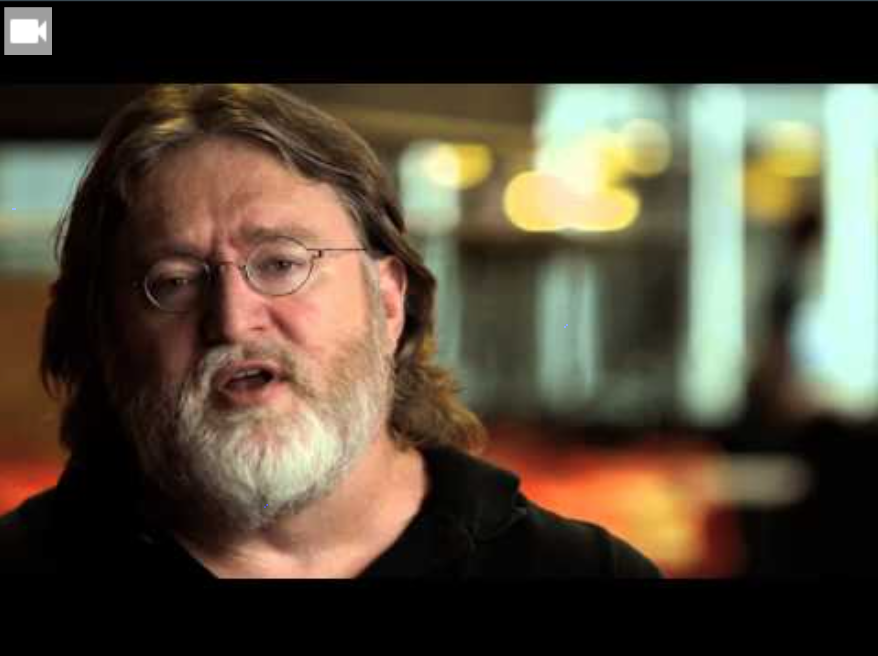
\includegraphics[scale=0.4]{img/why.png}}}
	\centerline{\colored{\href{https://www.youtube.com/watch?v=bKm-0VdTwA8}{https://www.youtube.com/watch?v=bKm-0VdTwA8}}}
\end{frame}

%%%%%%%%%%%%%%%%%%%%%%%%%%%%%%%%%%%%%%%%%%%%%%%%%%%%%

\begin{frame}{¿Qué es esta carrera? - Para TPI y LIDS}
  \small{
  Lo siguiente vale tanto para la \bolder{Tecnicatura en Programación
  Informática (TPI)} como en la \bolder{Licenciatura en Informática (LIDS)}.
  \begin{itemize}
    \item Ambas carreras buscan formar profesionales de la industria del software,
      enfocados al desarrollo de productos de software.
    \item Ambas se enfocan en escribir código fuente y producir programas.
    \item Ambas aspiran a generar profesionales capacitados que puedan desempeñarse de
      forma satisfactoria en la industria.
    \item Ninguna de ella se centra en el aprendizaje de un lenguaje de programación en
      particular, sino de conceptos, de ideas y procesos que van más allá de la
      herramienta utilizada.
    \item En ámbas van a ver varios lenguajes (Gobstones, Wollok, Smalltalk, Java,
      Python, Scala, JavaScript, Ruby, C, Haskell, entre otros) y van a ver como se
      reflejan los conceptos en dichos lenguajes.
    \item Un licenciado va a poder guiar equipos de trabajo, y encarar soluciones
      más complejas que un técnico.
  \end{itemize}
  }
\end{frame}

%%%%%%%%%%%%%%%%%%%%%%%%%%%%%%%%%%%%%%%%%%%%%%%%%%%%%

\begin{frame}{¿Qué NO es esta carrera? - Para TPI y LIDS}
  \small{\begin{itemize}
    \item No se centran en aprender herramientas (No es un curso corto para aprender a
      programar en una herramienta en particular)
    \item No están enfocadas a mantenimiento de infraestructura (armado de redes
      y servidores, etc). Si te interesa esa área, hacenoslo saber.
    \item No están enfocados en aprender herramientas informáticas y su uso
      (ej. hojas de cálculo, procesadores de texto, etc.)
    \item No está pensado para que sean programadores de juegos (aunque eso no
      quita que uno pueda dedicarse a eso luego, pues todas las herramientas
      aplican a esa industria también y de hecho hay alguna materia optativa de
      programación de juegos)
    \item No está pensado como vinculación de tecnología con arte, tal vez
      quieras mirar la \bolder{Licenciatura en Artes Digitales} o la
      carrera virtual \bolder{Licenciatura en Artes y Tecnologías}
  \end{itemize}
  \bolder{Si le parece que se anotó en la carrera equivocada, quedese igual,
    quien le dice, encuentra algo nuevo que le termina gustando más de lo que
    esperaba}
  }
\end{frame}

%%%%%%%%%%%%%%%%%%%%%%%%%%%%%%%%%%%%%%%%%%%%%%%%%%%%%

\begin{frame}{¿De qué voy a laburar? - Para TPI y LIDS}
  \small{
    En la Argentina, la industria del desarrollo de software es una industria
    ampliamente robusta, en constante crecimiento, y con una gran necesidad de
    mano de obra altamente calificada.
    \jump
    Como profesional va a poder desempeñarse como desarrollador de software en
    distintas empresas, tanto como parte de equipos de desarrollo (en especial los
    técnicos), como dirigiéndolos (en especial los licenciados).
    \jump
    Debido a la alta demanda y escasa oferta de profesionales calificados, es
    relativamente fácil conseguir empleo y los sueldos suelen ser generalmente
    buenos en comparación con otras industrias.
    \jump
    También puede desempeñarse como desarrollador freelance, haciendo trabajos
    de forma independiente, como monotributista o encarar sus propios proyectos
    e intentar venderlos por tu cuenta, aunque esto no siempre es fácil.
  }
\end{frame}

%%%%%%%%%%%%%%%%%%%%%%%%%%%%%%%%%%%%%%%%%%%%%%%%%%%%%

\begin{frame}{¿Qué es esta carrera? - Para Bioinformática}
  \small{
  Lo siguiente vale para la \bolder{Licenciatura en Bioinformática}.
  \jump
  La Licenciatura en Bioinformática de la Universidad Nacional de Quilmes (UNQ)
  tiene como principal objetivo la formación de profesionales dedicados a la
  investigación, el desarrollo y/o la aplicación de herramientas informáticas a
  la solución de problemas biológicos (en sentido amplio), médicos o
  biotecnológicos. El conjunto de problemas biológicos a solucionar incluye
  aquellos que impliquen la adquisición, almacenaje, recuperación, organización,
  análisis y visualización de datos. Todos estos aspectos están íntimamente
  ligados a la transformación de los datos en información y conocimiento útil
  y necesario para el bienestar de la sociedad en su conjunto.
  }
\end{frame}

%%%%%%%%%%%%%%%%%%%%%%%%%%%%%%%%%%%%%%%%%%%%%%%%%%%%%

%\begin{frame}{¿Qué NO es esta carrera? - 2}
  % Estaría bueno hablar con alguien de bioinformatica para ver que cosas NO es
  % en particular, como se diferencia de biotecnologia
%\end{frame}

%%%%%%%%%%%%%%%%%%%%%%%%%%%%%%%%%%%%%%%%%%%%%%%%%%%%%

%\begin{frame}{¿De qué voy a laburar? - 2}
  %  Idem anterior, dar ejemplos de laburo posta
%\end{frame}

%%%%%%%%%%%%%%%%%%%%%%%%%%%%%%%%%%%%%%%%%%%%%%%%%%%%%

\begin{frame}[plain]
	\centerline{\bolder{\Large{¿Consultas?}}}
  \centerline{Hable ahora o calle para siempre.}
  ~\jump
  \small{No, mentira, puede consultar luego, pero lo ideal es que
    consulte cuanto antes y no que espere a último momento para hacerlo, pues
    puede ser tarde y más complicado de resolver problemas puntuales.}
\end{frame}

%%%%%%%%%%%%%%%%%%%%%%%%%%%%%%%%%%%%%%%%%%%%%%%%%%%%%

\begin{frame}[plain]
  \bolder{\Huge\centerline{¡¡¡BIENVENIDOS/AS!!!}}
  \centerline{Que comience la materia.}
\end{frame}

%%%%%%%%%%%%%%%%%%%%%%%%%%%%%%%%%%%%%%%%%%%%%%%%%%%%%
